\clearpage
\chapter{Sample SGA Fitness Distributions}
\label{appendix:SGAFitness}

This appendix contains some sample SGA fitness distributions. As was discussed
in Section~\ref{6_SGA}, the distributions appear to be normal, but quickly show
as skewed character which can be seen in these figures.

\clearpage
\begin{figure}[htp]
\centerline{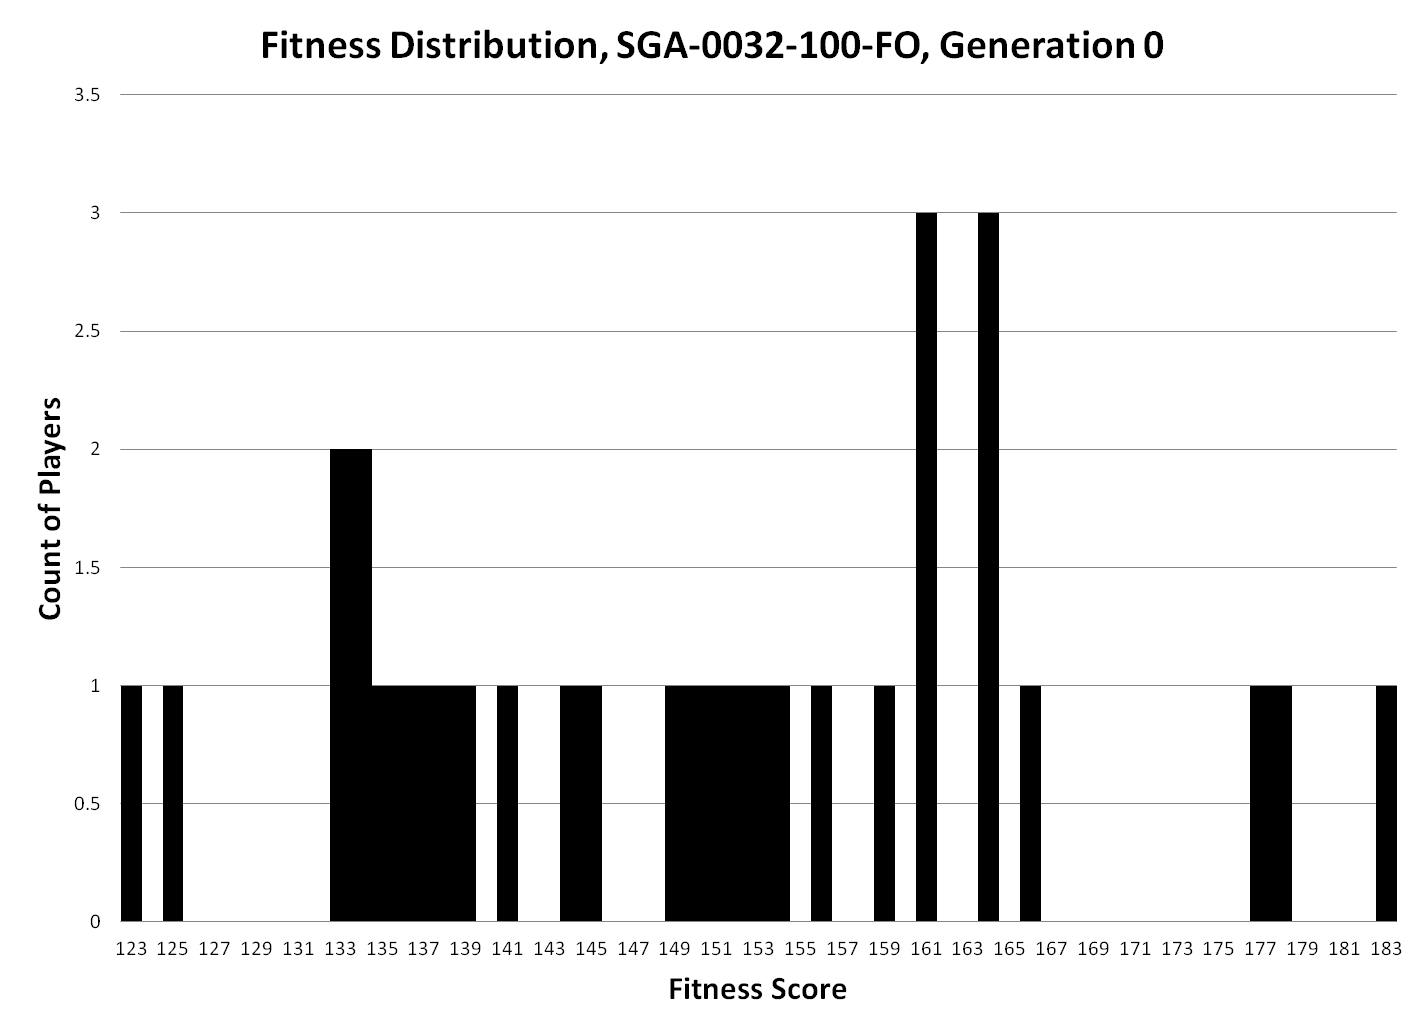
\includegraphics[width=0.75\columnwidth]{Figures/SGA_0032_100_FO_gen000.png}}
\caption{Fitness Distribution, SGA-0032-100-FO, Generation 0}
\end{figure}

\begin{figure}[htp]
\centerline{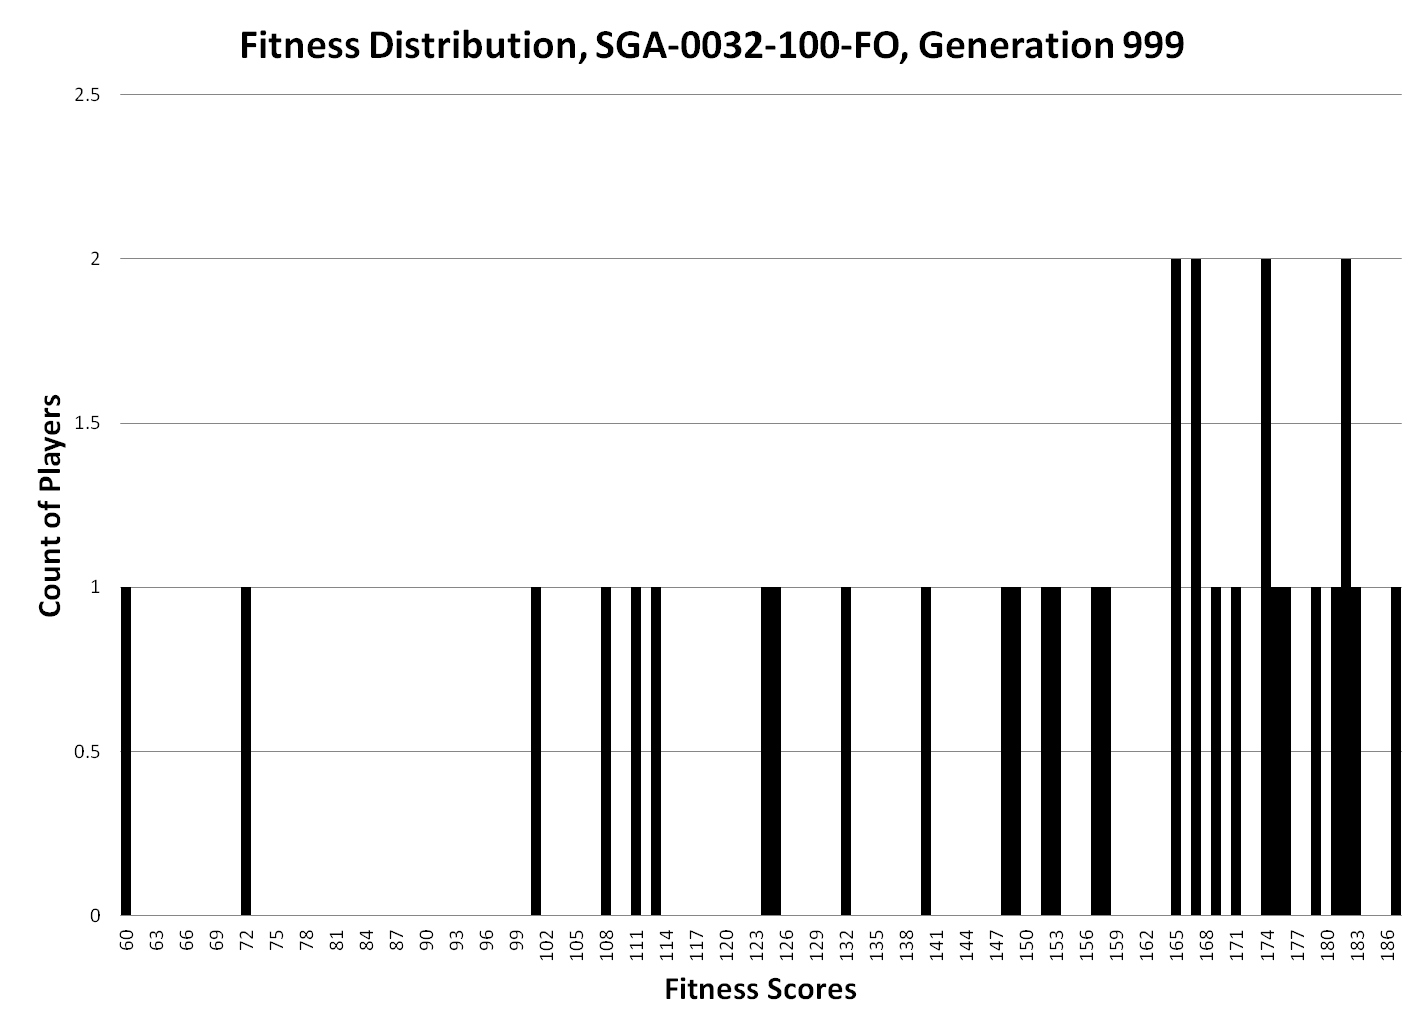
\includegraphics[width=0.75\columnwidth]{Figures/SGA_0032_100_FO_gen999.png}}
\caption{Fitness Distribution, SGA-0032-100-FO, Generation 999}
\end{figure}

\begin{figure}[htp]
\centerline{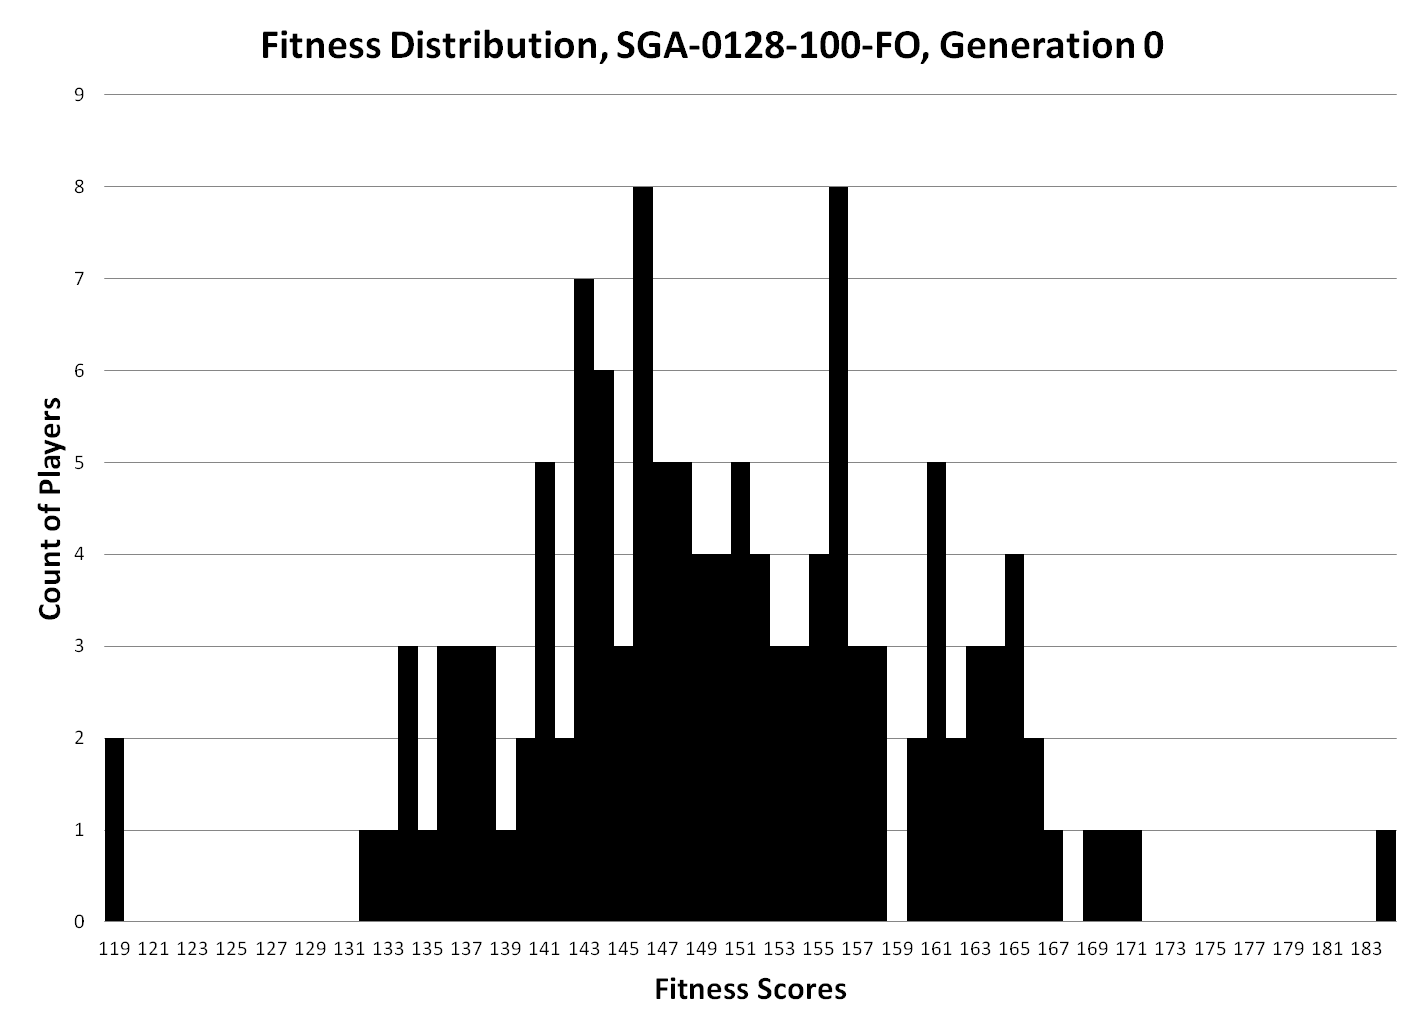
\includegraphics[width=0.75\columnwidth]{Figures/SGA_0128_100_FO_gen000.png}}
\caption{Fitness Distribution, SGA-0128-100-FO, Generation 0}
\end{figure}

\begin{figure}[htp]
\centerline{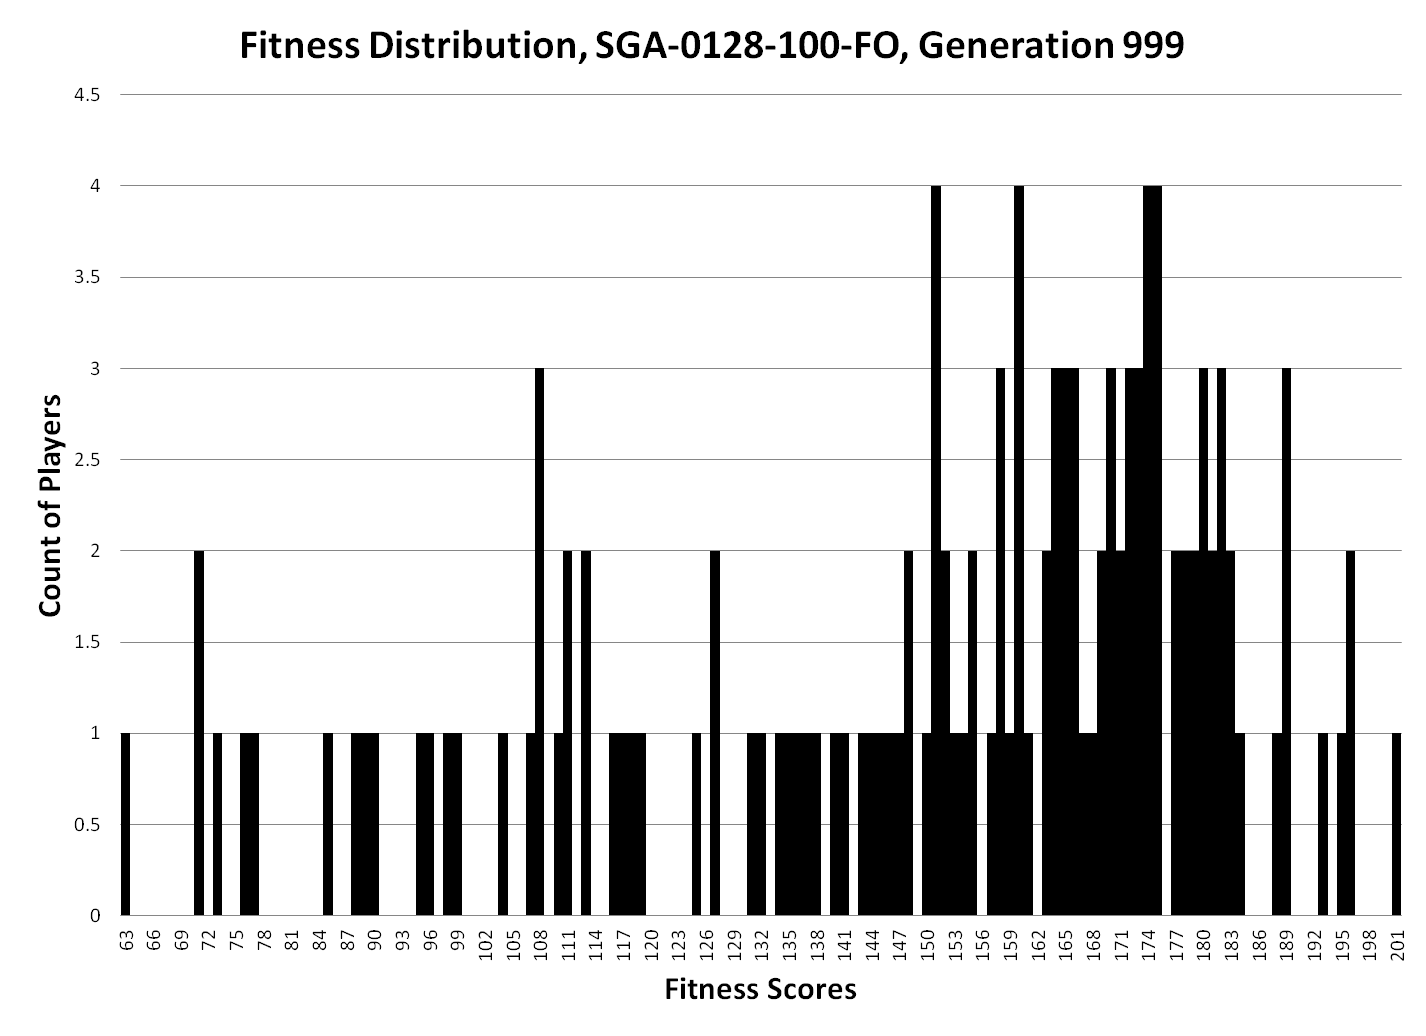
\includegraphics[width=0.75\columnwidth]{Figures/SGA_0128_100_FO_gen999.png}}
\caption{Fitness Distribution, SGA-0128-100-FO, Generation 999}
\end{figure}

\begin{figure}[htp]
\centerline{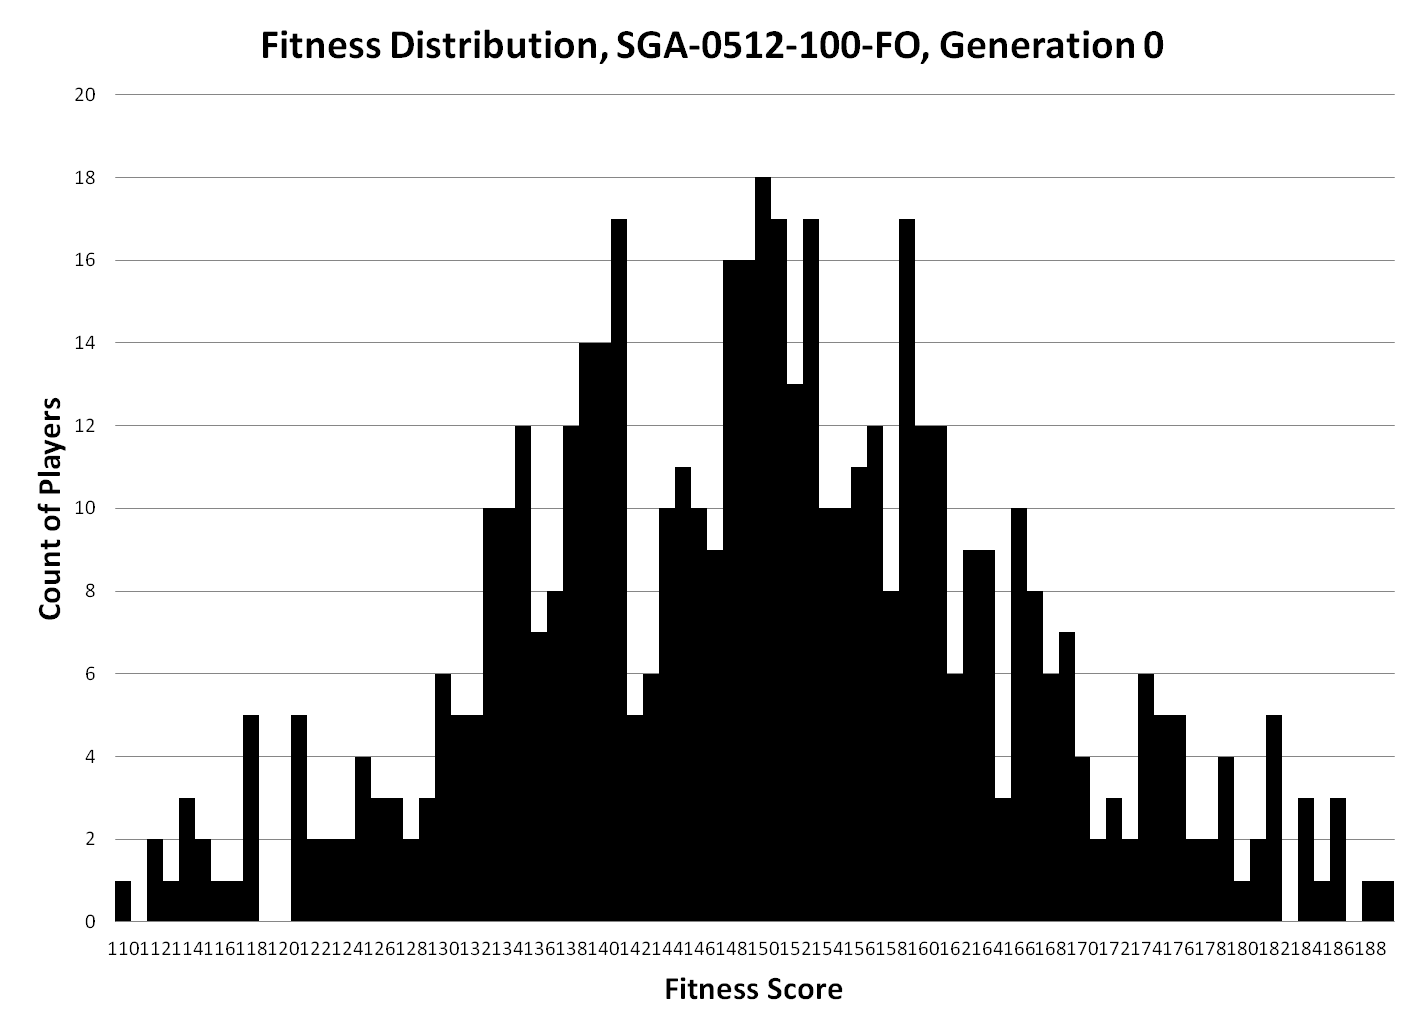
\includegraphics[width=0.75\columnwidth]{Figures/SGA_0512_100_FO_gen000.png}}
\caption{Fitness Distribution, SGA-0512-100-FO, Generation 0}
\end{figure}

\begin{figure}[htp]
\centerline{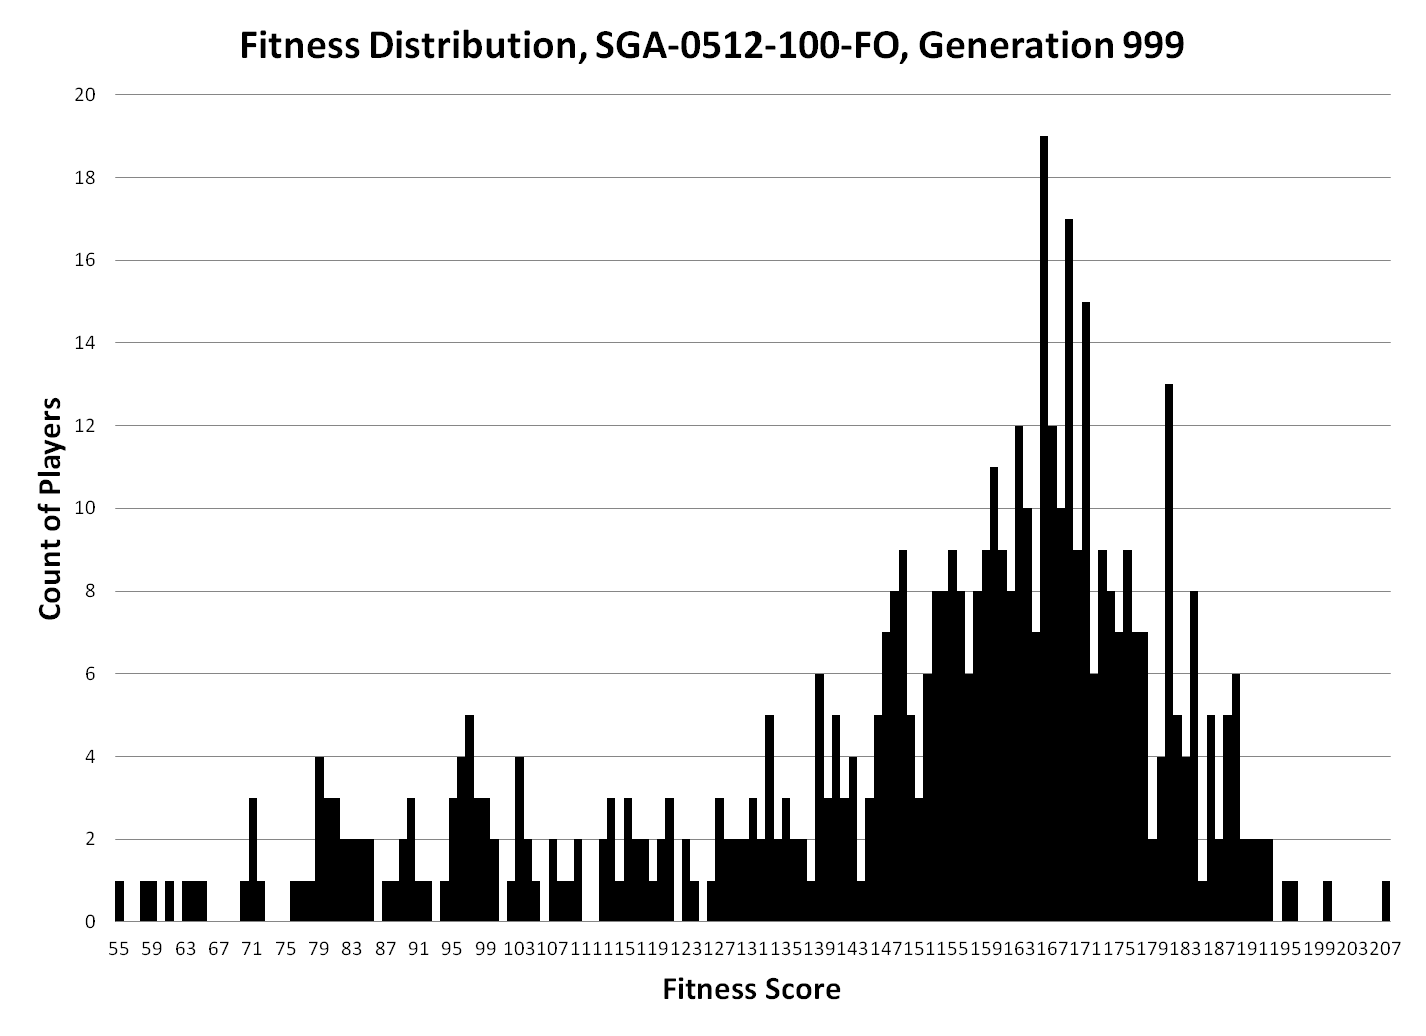
\includegraphics[width=0.75\columnwidth]{Figures/SGA_0512_100_FO_gen999.png}}
\caption{Fitness Distribution, SGA-0512-100-FO, Generation 999}
\end{figure}

\begin{figure}[htp]
\centerline{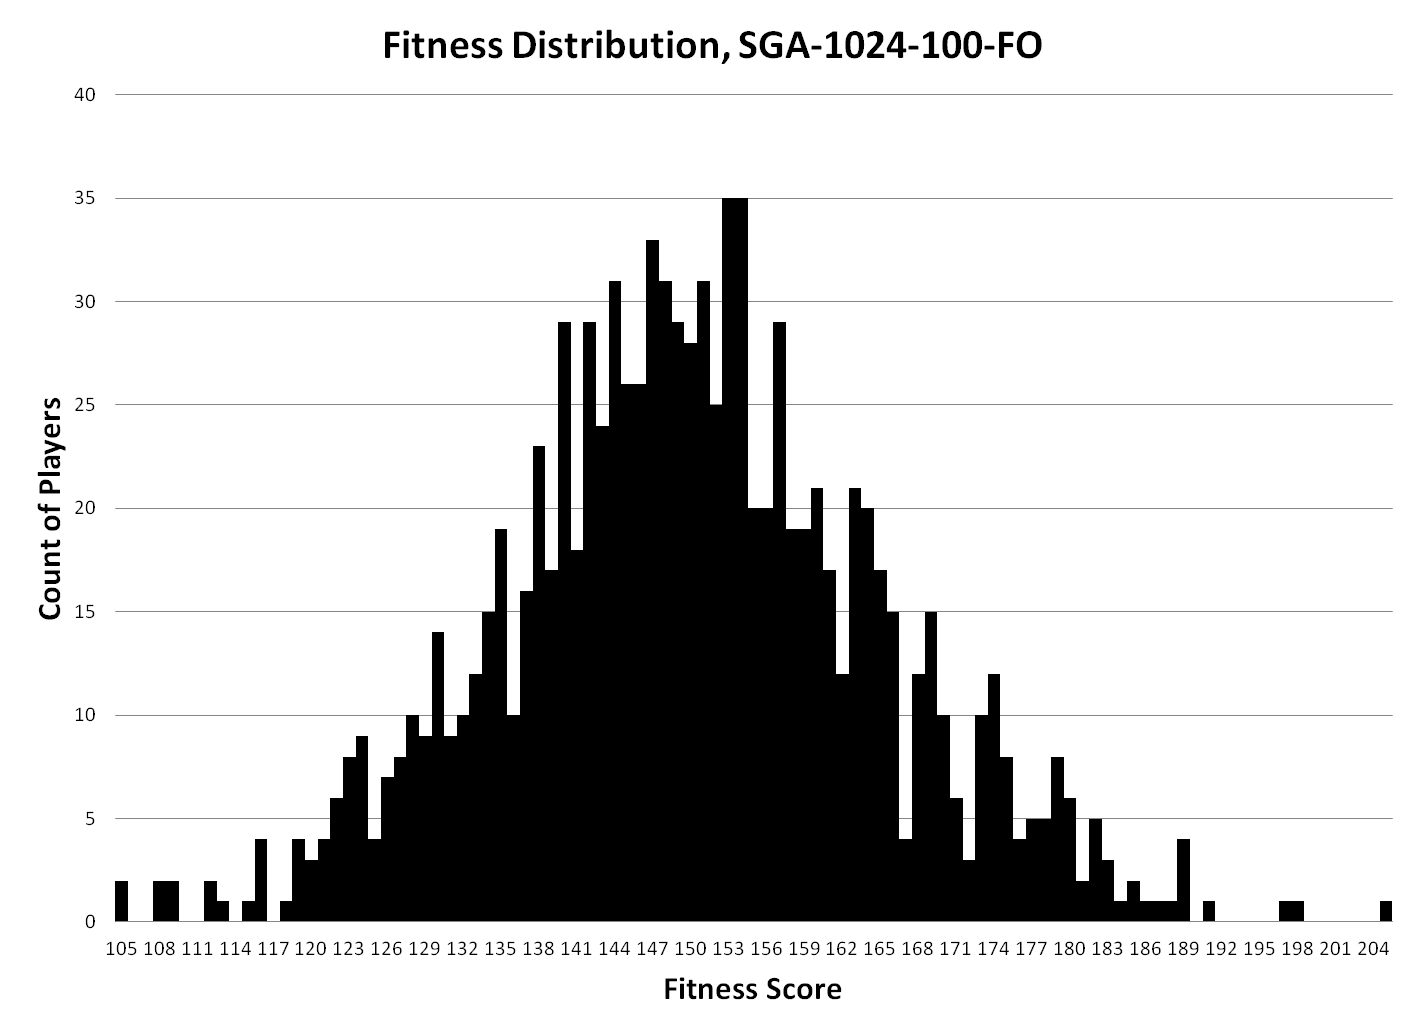
\includegraphics[width=0.75\columnwidth]{Figures/SGA_1024_100_FO_gen0.png}}
\caption{Fitness Distribution, SGA-1024-100-FO, Generation 0}
\end{figure}

\begin{figure}[htp]
\centerline{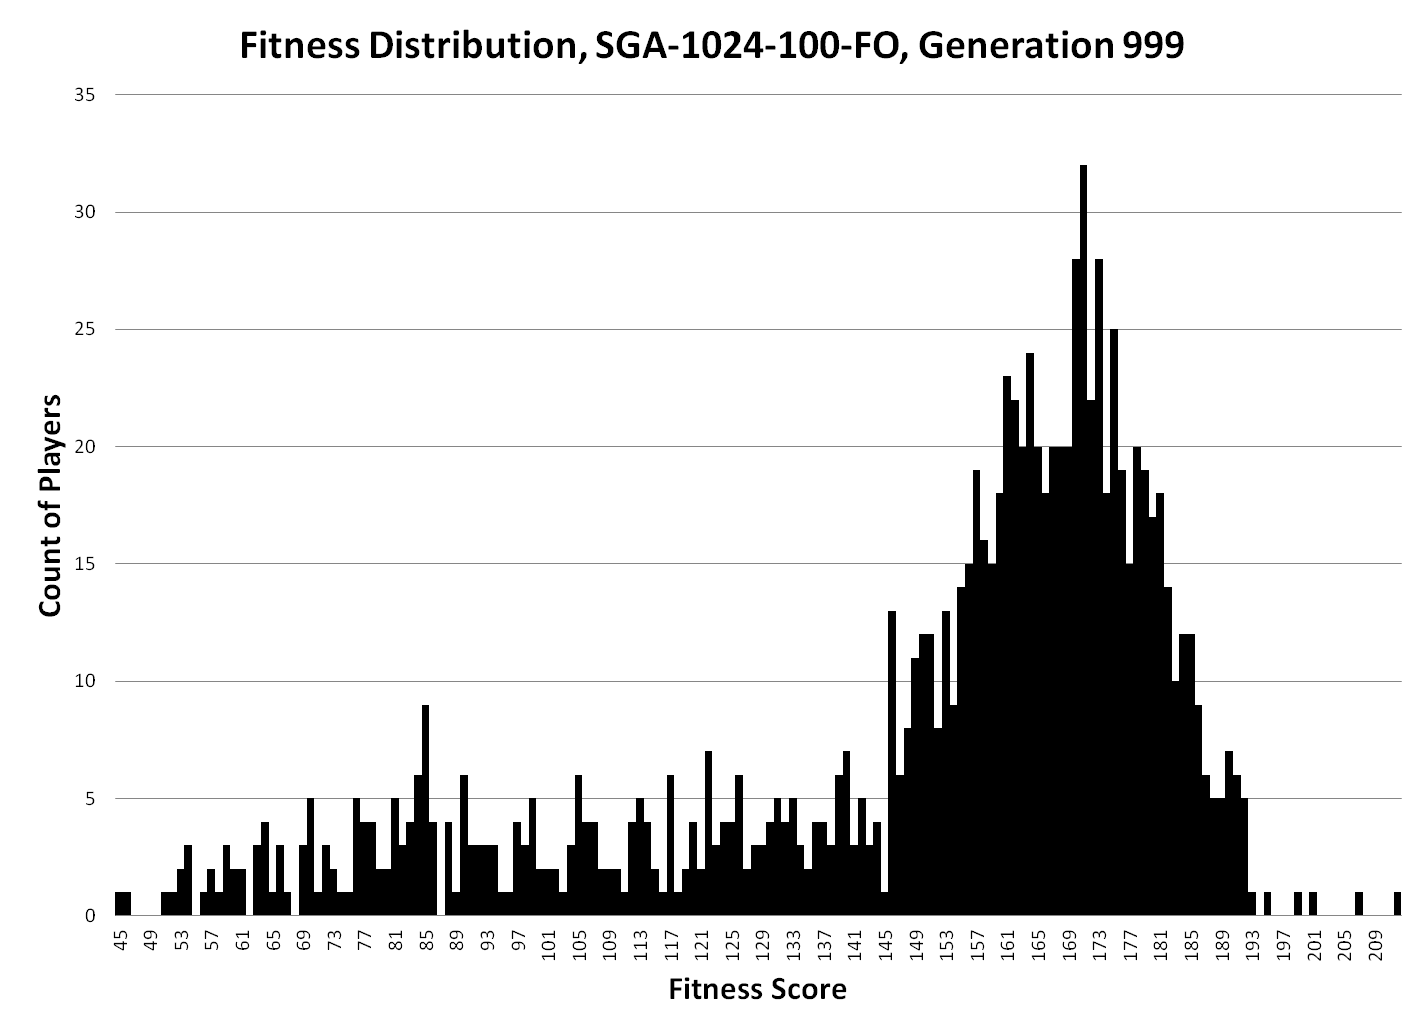
\includegraphics[width=0.75\columnwidth]{Figures/SGA_1024_100_FO_gen999.png}}
\caption{Fitness Distribution, SGA-1024-100-FO, Generation 999}
\end{figure}
